\documentclass[tikz, border=15pt]{standalone}
\usepackage{tikz}
\usetikzlibrary{arrows.meta, positioning, shapes.geometric, calc}
\usepackage{amsmath, lmodern}
\usepackage[T1]{fontenc}

\tikzset{
  script/.style = {draw, rectangle, rounded corners=3pt, thick,
                   minimum width=4.0cm, minimum height=0.85cm,
                   align=center, font=\small\ttfamily},
  data/.style   = {draw, trapezium, trapezium left angle=75, trapezium right angle=105,
                   thick, fill=yellow!8,
                   minimum width=3.0cm, minimum height=0.7cm,
                   align=center, font=\small\ttfamily},
  hw/.style     = {draw, rectangle, rounded corners=10pt, thick,
                   fill=green!6, dashed,
                   minimum width=3.6cm, minimum height=0.75cm,
                   align=center, font=\small},
  note/.style   = {font=\footnotesize\itshape, gray!70, anchor=west},
  arr/.style    = {->, >=Stealth, thick, shorten >=1pt, shorten <=1pt},
}

\begin{document}
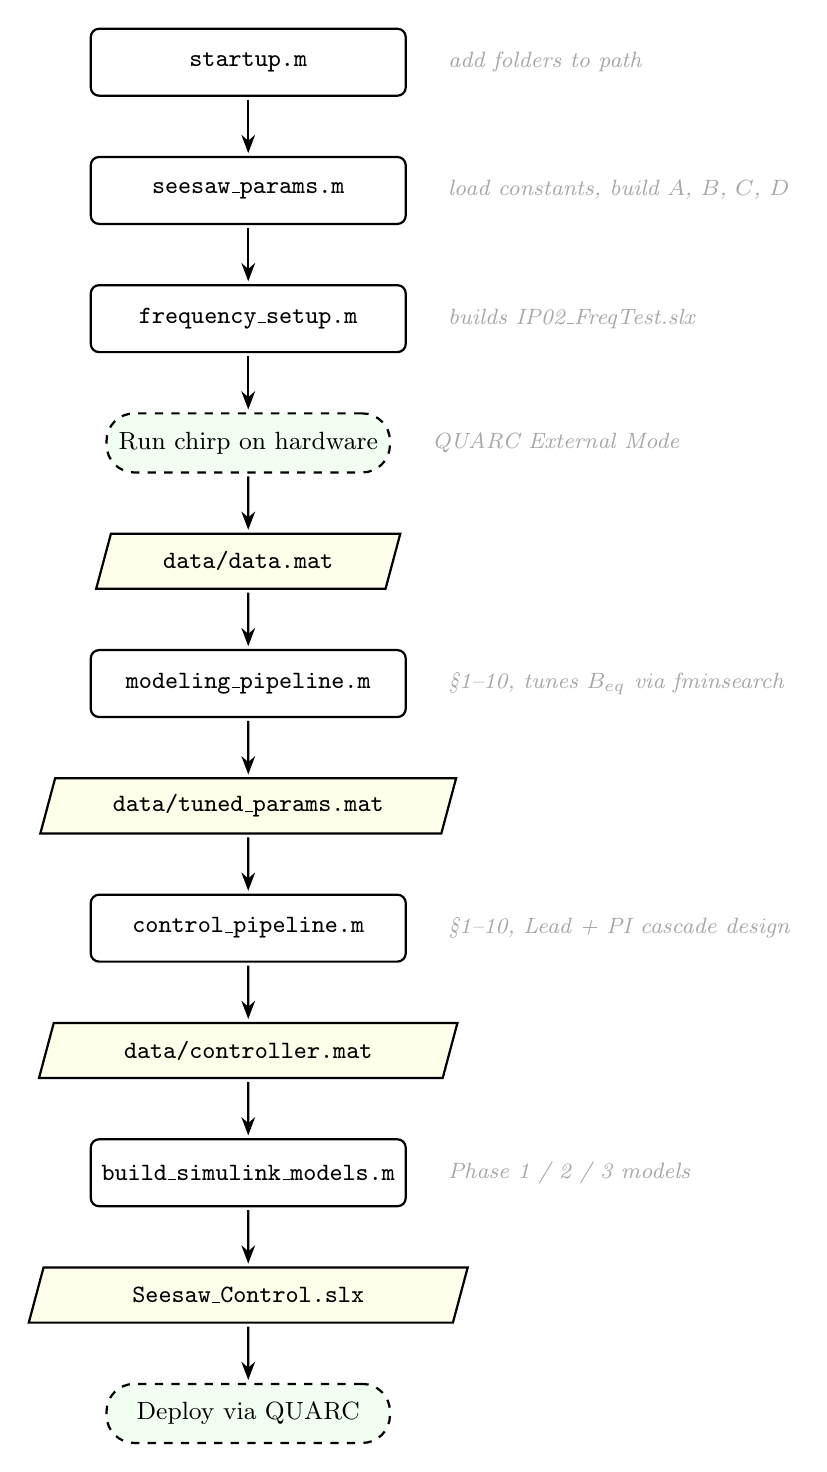
\begin{tikzpicture}[node distance=0.75cm]

  \node[script]                           (startup) {startup.m};
  \node[script, below=of startup]         (params)  {seesaw\_params.m};
  \node[script, below=of params]          (fsetup)  {frequency\_setup.m};
  \node[hw,     below=of fsetup]          (hw1)     {Run chirp on hardware};
  \node[data,   below=of hw1]             (dmat)    {data/data.mat};
  \node[script, below=of dmat]            (mpipe)   {modeling\_pipeline.m};
  \node[data,   below=of mpipe]           (tmat)    {data/tuned\_params.mat};
  \node[script, below=of tmat]            (cpipe)   {control\_pipeline.m};
  \node[data,   below=of cpipe]           (cmat)    {data/controller.mat};
  \node[script, below=of cmat]            (build)   {build\_simulink\_models.m};
  \node[data,   below=of build]           (slx)     {Seesaw\_Control.slx};
  \node[hw,     below=of slx]             (hw2)     {Deploy via QUARC};

  %% Arrows
  \draw[arr] (startup) -- (params);
  \draw[arr] (params)  -- (fsetup);
  \draw[arr] (fsetup)  -- (hw1);
  \draw[arr] (hw1)     -- (dmat);
  \draw[arr] (dmat)    -- (mpipe);
  \draw[arr] (mpipe)   -- (tmat);
  \draw[arr] (tmat)    -- (cpipe);
  \draw[arr] (cpipe)   -- (cmat);
  \draw[arr] (cmat)    -- (build);
  \draw[arr] (build)   -- (slx);
  \draw[arr] (slx)     -- (hw2);

  %% Side annotations
  \node[note] at ($(startup.east)+(0.4,0)$)  {add folders to path};
  \node[note] at ($(params.east)+(0.4,0)$)   {load constants, build $A$, $B$, $C$, $D$};
  \node[note] at ($(fsetup.east)+(0.4,0)$)   {builds IP02\_FreqTest.slx};
  \node[note] at ($(hw1.east)+(0.4,0)$)      {QUARC External Mode};
  \node[note] at ($(mpipe.east)+(0.4,0)$)    {\S1--10, tunes $B_{eq}$ via fminsearch};
  \node[note] at ($(cpipe.east)+(0.4,0)$)    {\S1--10, Lead + PI cascade design};
  \node[note] at ($(build.east)+(0.4,0)$)    {Phase 1 / 2 / 3 models};

\end{tikzpicture}
\end{document}
